\documentclass[10pt, a4paper, onecolumn]{scrartcl}
\usepackage{cite}  
\usepackage{times}
\usepackage{amsmath}
\usepackage{amsfonts}
\usepackage{amssymb}
\usepackage{graphicx}
\usepackage{listings}
\usepackage{enumitem} % used for list - no spaces between items
\usepackage[english]{babel} % English language/hyphenation
\usepackage[top=2cm, bottom= 3.2cm, left=2cm, right=2cm, columnsep=0.6cm]{geometry}
\usepackage{color} %red, green, blue, yellow, cyan, magenta, black, white
\definecolor{mygreen}{RGB}{28,172,0} % color values Red, Green, Blue
\definecolor{mylilas}{RGB}{170,55,241}
\usepackage{fancyhdr}
\pagestyle{fancyplain}
\fancyhead{}
\renewcommand{\headrulewidth}{0pt} % Remove header underlines
\fancyfoot[L]{} % Empty left footer
\fancyfoot[C]{} % Empty center footer
\fancyfoot[R]{\thepage} 
\usepackage{tikz}
\usetikzlibrary{shapes.geometric,arrows}

\usepackage{sectsty} % Allows customizing section commands
\sectionfont{\centering\large\textbf}
\subsectionfont{\flushleft\normalsize\normalfont\textbf}
\subsubsectionfont{\flushleft\normalsize\normalfont\textit}
%\allsectionsfont{\centering} % Make all sections centered

\setlength\parindent{0pt} % remove all indentations in document

%----------------------------------------------------------------------------------------
%	BEGIN DOCUMENT
%----------------------------------------------------------------------------------------
\newcommand{\horrule}[1]{\rule{\linewidth}{#1}}

\begin{document}
	
	\title{\normalfont \normalsize
		\textsc{University of Witwatersrand, Department of Electrical Engineering} \\ [10pt]
		\horrule{0.5pt} \\ [10pt]
		\huge Software Requirement Specification for Shopping Route Recommender \\
		\horrule{2pt} \\ [10pt]}
	\author{\textbf{\normalsize{Luka Cakic (671913), Ronen Freeman (386910), Devin Taylor (603956) and Matthew Marsden (609293)}} \\ [10pt]}
	\date {\normalsize \today}
	
	\maketitle
	
	
	\section{Introduction}
	
		\subsection{Purpose}
		
		\subsection{Document Conventions}
		
		\subsection{Intended Audience and Reading Suggestions}
		
		\subsection{Project Scope}
		
		\subsection{References}
	
	\section{Overall Description}
	
		\subsection{Product Perspective}
		
			The Shopping Route Recommender is an application used by consumers to maximise their shopping experience in terms of three preferred optimisations: minimum cost, travel distance and travel time. The consumer is able to log onto a Website or Smartphone application and create a shopping list with a desired route being generated.  Enabling a user to optimise their shopping experience is a potential success from the start, as their daily routines can become more efficiently and effectively undertaken. The application's use is not only restricted to the general public, but can also be used by businesses and companies involved in the stock collection courier service industries. The application is aimed at being user friendly, simple, and interactive with maximum customisation being a priority aspect in order to maximise an individuals needs. 
		
		\subsection{Product Features}
		
			The list of product features below aim to provide an easy-to-use, customizable application interface for all users. 
		
			\begin{itemize}
				\item Interactive shopping list menu.
				\begin{itemize}
					\item add or remove item
				\end{itemize}
				\item Interactive optimisation selection options.
				\begin{itemize}
					\item minimise cost
					\item minimise travel time
					\item minimise travle distance
				\end{itemize}
				\item Interactive shopping area selection options.
				\begin{itemize}
					\item select from a number of suburbs or regions
				\end{itemize}
				\item Interactive route map displaying alternate routes for selection.
				\begin{itemize}
					\item rotate map
					\item slide map
					\item zoom in/out
					\item satellite view
				\end{itemize}
			\end{itemize}
		
		\subsection{User Classes and Characteristics}
		
			The application is aimed for the general public's use as well as certain business industries. 
			
			\begin{itemize}
				\item General Public
				\begin{itemize}
					\item General population wanting to buy their routine shopping list
					\item General population looking for more specific products and their preferred optimised route
					\item Foreign individuals looking for their ideal shopping locations or travel routes
				\end{itemize}
				\item Business Industries
				\begin{itemize}
					\item Courier companies collecting stock or products from various distributors/stores
				\end{itemize}
			\end{itemize}
		
		\subsection{Operating Environment}
		
			Shopping Route Recommender is an application designed to run on the most Web Browsers as well on Google Android and Mac OS X Smartphones. 
			
			\begin{itemize}
				\item Software Requirements
				\begin{itemize}
					\item Internet connectivity
					\item Entry level Smartphone
					\item Mozilla Firefox, Microsoft Edge, Google Chrome, Microsoft Explorer, Safari
				\end{itemize}
				\item Hardware Requirements
				\begin{itemize}
					\item Entry level Smartphone with interactive touch screen
				\end{itemize}
			\end{itemize}
		
		\subsection{Design and Implementation Constraints}
		
			Shopping Route Recommender is platform independent and is written in \textcolor{red}{language}. In addition, Google Maps API is implemented for generating the desired optimised shopping route. The accuracy of the generated route and optimisation algorithms is therefore dependent on the accuracy of the Google Maps detailing. 
		
		\subsection{User Documentation}
		
		   	A general help and FAQ menu will be provided within the application. This will function as the "user manual" of the application. 
		
		\subsection{Assumptions and Dependencies}
	
	\section{System Features}
	
		Shopping Route Recommender was designed with user experience as its primary concern. As a result of this the product features are simplistic in nature in order to provide the customer with only the essentials.	This section provides a detailed description of each system features in order to make future system extensions as easy as possible. 
	
		\subsection{System Feature 1 - Adding items to shopping cart}
		\label{featureadd}
		
			\subsubsection{Description}
			
				The Shopping Route Recommender's primary feature is for the user to be able to continuously add shopping items to their cart. The user will be able to continuously log into the application and add items to the shopping cart on an add-hock basis. These items will remain in the basket until such time that the user wants to go shopping. 
			
			\subsubsection{Stimulus/Response Sequences}
			
				The user will click in the "Add Items" field at which point a list will be displayed that will contain all previously added items listed one after the other (in the order in which they were added). Within this list the user will be able to complete one of the following actions:
				
				\begin{itemize}
					\item Add new item - The user will be able to select the "Add new item" button in order to be allowed to enter a new item. 
					\item Remove existing item - The user will be able to select the cross new to a specific item at which point the item will be removed from the shopping list.
					\item Edit existing item - The user will be able to make modifications to the description of an existing item.
				\end{itemize}
			
			\subsubsection{Functional Requirements}
			
				\begin{itemize}
					\item The user can only add a single item at a time.
					\item The user can only remove a single item at a time.
					\item The user can only edit a single item at a time.
				\end{itemize}
			
		
		\subsection{System Feature 2 - Upload Existing List}
			
			\subsubsection{Description}
			
				The developers acknowledge the fact that not all users will have continuous access to internet and thus the ability to access the above mentioned shopping list. The proposed solution was to allow the user to add items to a .csv file and upload this only when they actual want to go shopping. 
				
			\subsubsection{Stimulus/Response Sequences}
			
				On the home page there is a "Upload Shopping List" button. Once the user clicks on this button the user will be required to provide the path to the .csv document. Once the path has been provided the user will be required to click on the upload button and the .csv file will be imported. Upon completion the user will be able to access, and interact with, the shopping list as mentioned in Section~\ref{featureadd}.
		
		\subsection{System Feature 3 - Add Location}
				
			\subsubsection{Description}
			
				In order for the route to be provided it is required that the application know the user's location. 
				
			\subsubsection{Stimulus/Response Sequences}
			
				The user is presented with a "Add Location" option on the home screen. Upon selecting this option the user has the ability to make their location known in two different ways:
				
				\begin{itemize}
					\item Entering their location manually.
					\item Finding their location through the use of the Google Maps API.
				\end{itemize}
				
				The primary motivation behind allowing the user to manually enter their location is that not all users will have access to GPS and thus will be able to find their location.\\
				
				The location entered at this point is the same location that will be used as the starting position for the route that is planned when the "Generate Route" option is selected.
				
			\subsubsection{Functional Requirements}
			
				\begin{itemize}
					\item In order to use the "find my location" option the user is required to have GPS access.
				\end{itemize}
				
		\subsection{System Feature 4 - Preferred Optimisation}
		
			\subsubsection{Description}
			
				A decision was made in order to allow the user to have control of the nature of the route that they will follow. This was due to the fact that multiple customers will view different aspects as their primary concern. In other words, some users might value the cost of things over the distance required to travel, while for other the cost of things may not be of concern.
			
			\subsubsection{Stimulus/Response Sequences}
			
				On the home page there is a "Preffered Optimisation" drop down menu. Once the user selects the "Preffered Optimisation" drop-down menu they will be provided with the following options:
				
				\begin{itemize}
					\item Fastest Route - The user will be allowed to select that they would like to take the fastest possible route in order to obtain all the items on their shopping list. The primary contributor to delays will be traffic.
					\item Shortest Route - The user will be allowed to select that they would like to travel the shortest possible distance in order to obtain all the items on their shopping list. This selection will not incorporate traffic information.
					\item Cheapest Total Cost - The optimisation will primarily consider the cost of items at the expense of the distance required to be travelled in order to obtain these items. 
				\end{itemize}
				
				The user will also be provided with all alternative routes and they time expense that would be incurred if they select to take the alternate routes. The route distance optimisation will primarily be achieved through the use of the Google Maps API.
			
			\subsubsection{Functional Requirements}
			
				\begin{itemize}
					\item The application is required to link to the Google Maps API.
					\item The user is required to have GPS activated on their mobile device if they wish to use navigation.
				\end{itemize}
		
		\subsection{System Feature 5 - Generate Route}
		
			\subsubsection{Description}
			
				The generate route option incorporates all the above mentioned features and provides the user the with the preferred route. 
				
			\subsubsection{Stimulus/Response Sequences}
			
				Upon selection of the "Generate Route" option the user will be directed to a page that contains the Google Map with the route drawn onto it as well as a set of directions in order to allow for off-line use. If the user would prefer to navigate using a mobile device they will be able to do so through the use of Google Maps.
				
			\subsubsection{Functional Requirements}
			
				\begin{itemize}
					\item Access to Google Maps API is required.
				\end{itemize}
				
	
	\section{External Interface Requirements}
	
		\subsection{User Interfaces - GUI}
		
		
				The Shopping Route Recommender (SRRec) GUI is simple to use and designed such that the user is able to access all the main features easily. The interface communicates with the data layer which then incorporates Googles' API to deliver the most accurate and optimised shopping route. . Furthermore the application is easily portable between devices of different screen sizes, in that the content on the pages automatically adjust to fit the appropriate screen.\\
				
				The most common features of SSRec's GUI are:
				
				\begin{itemize}
					\item The sidebar menu accessible from all the subsequent pages:
					\begin{figure}[h!]
						\centering
						
\includegraphics[scale = 0.495]{Images/menu.png}
						\label{menu}
					\end{figure}
					
					\item The landing page and main application window where a user inputs their shopping list, location and preffered optimisation from which the application generates an optimised route:
					\begin{figure}[h!]
						\centering
						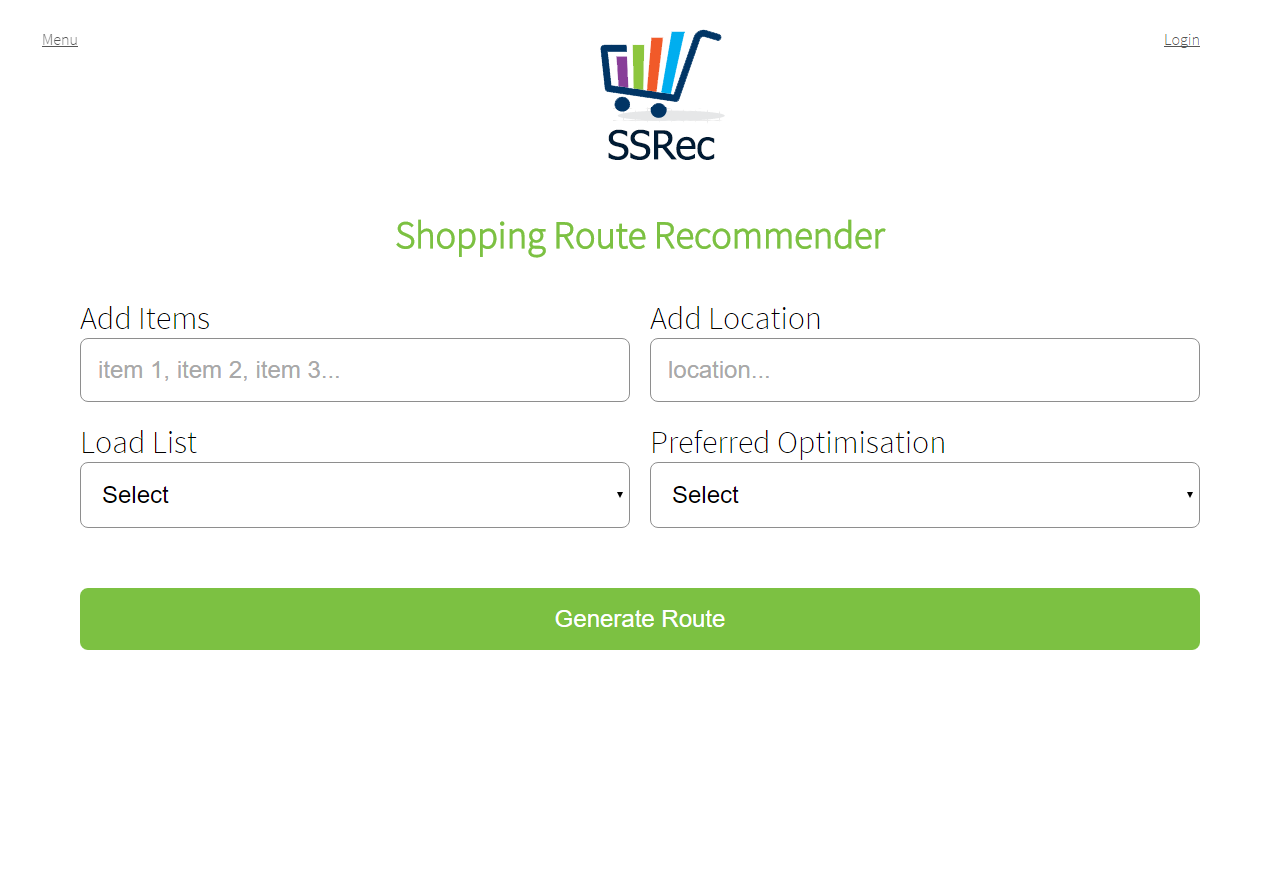
\includegraphics[scale = 0.5]{Images/index.png}
						\label{menu}
					\end{figure}
					
					\item Route and Directions page generated after a user has input their shopping list, location and preferred optimisation:
					\begin{figure}[h!]
						\centering
						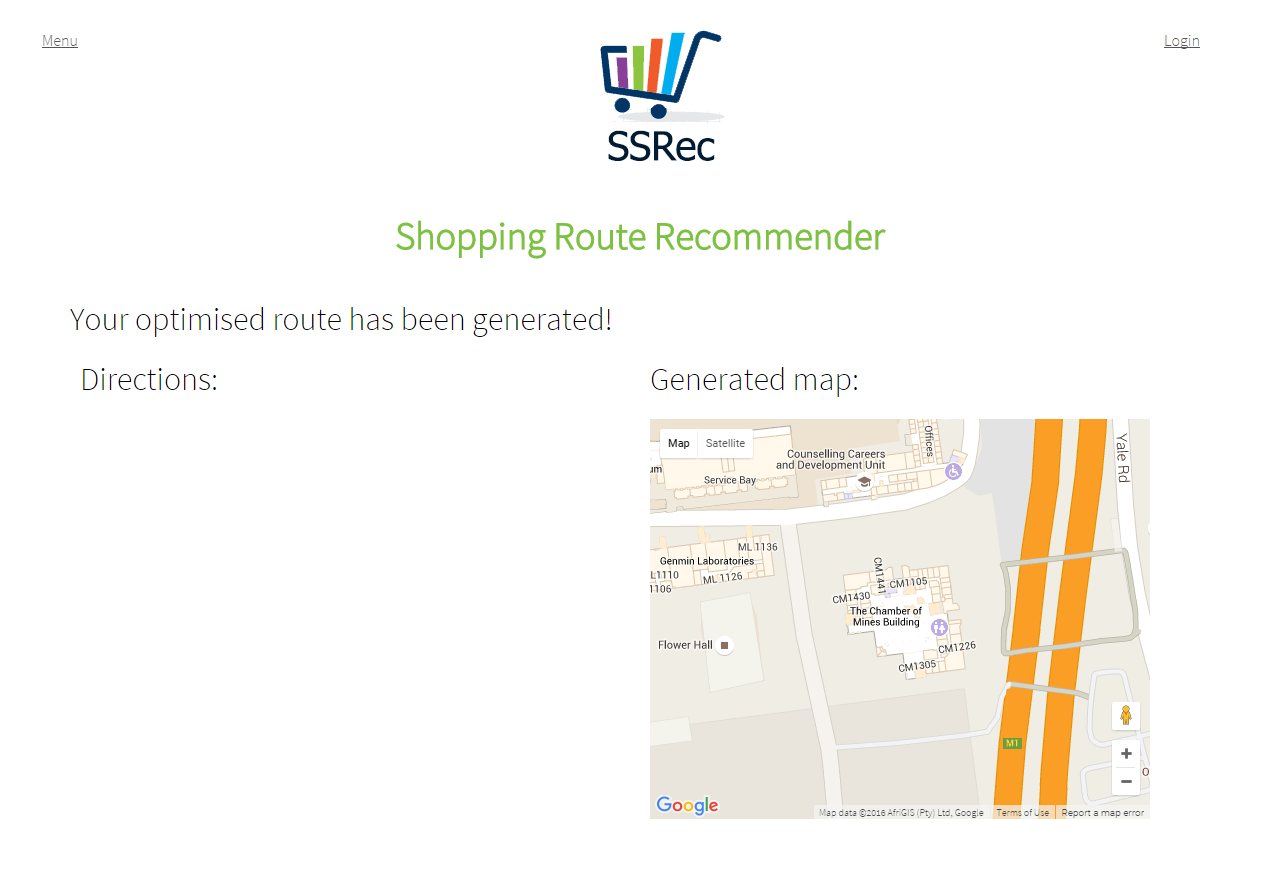
\includegraphics[scale = 0.5]{Images/routeGen.png}
						\label{menu}
					\end{figure}
					
					\item The page where a user can either login or create a new account:
					\begin{figure}[h!]
						\centering
						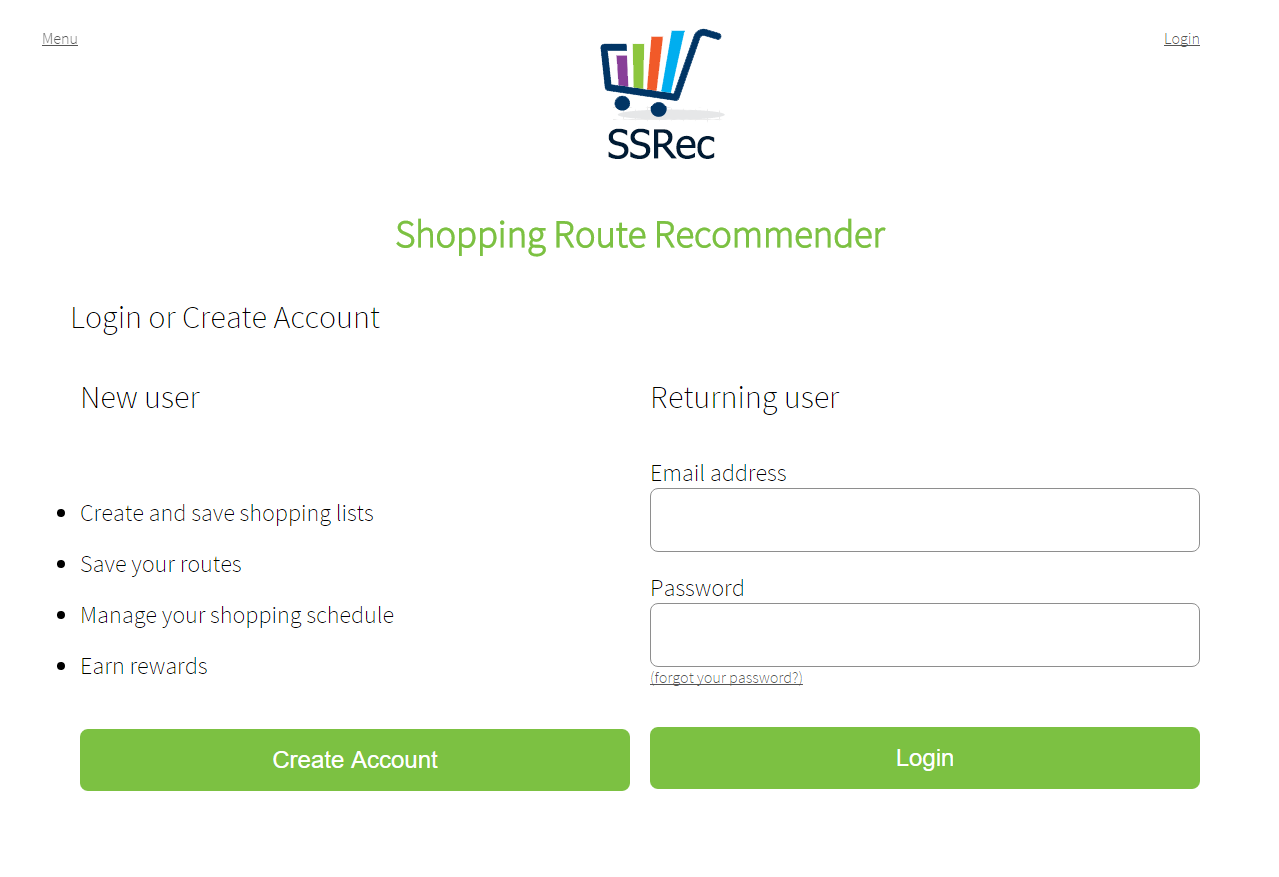
\includegraphics[scale = 0.5]{Images/login.png}
						\label{menu}
					\end{figure}
					
					\vspace{-12mm}
					\item The page where a new user can create an account:
					\begin{figure}[h!]
						\centering
						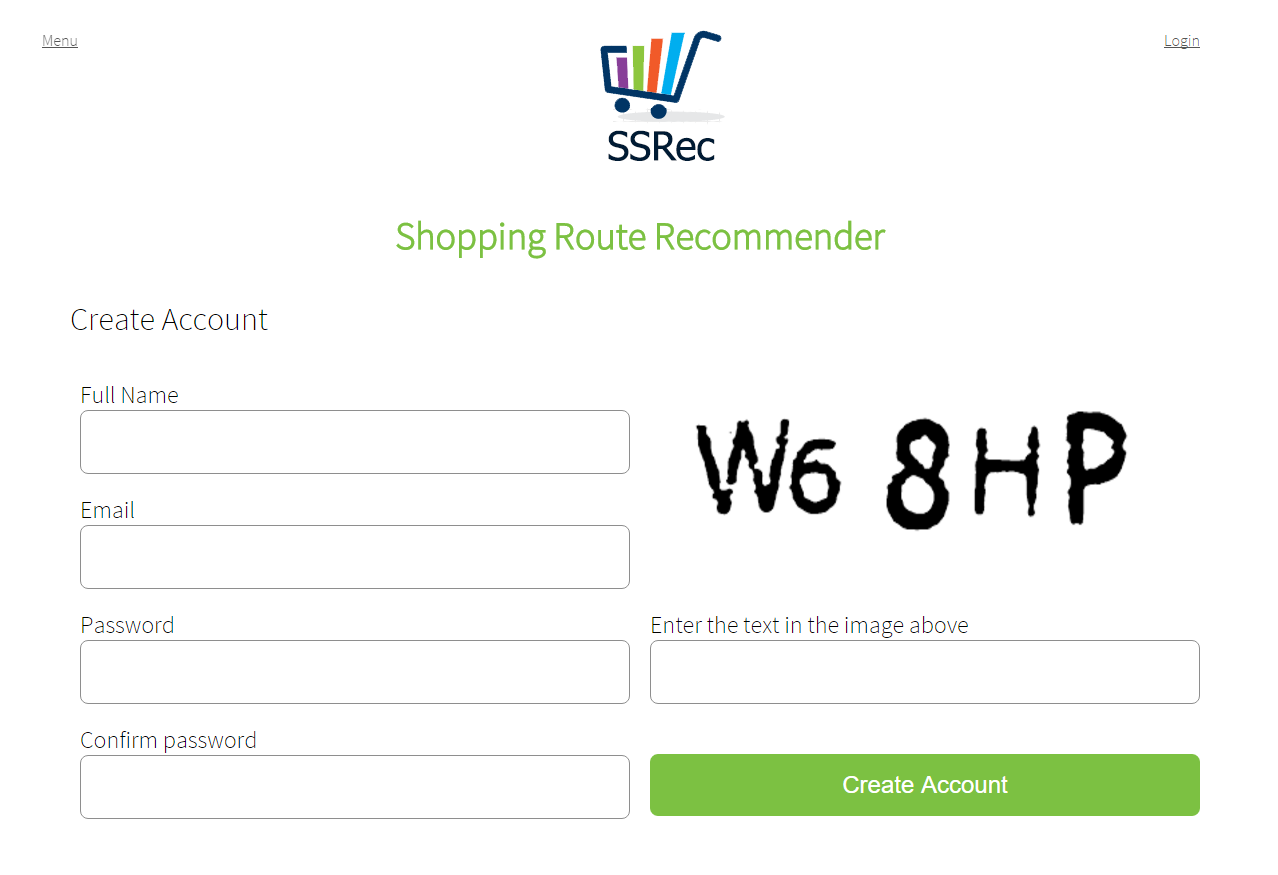
\includegraphics[scale = 0.5]{Images/createAccount.png}
						\label{menu}
					\end{figure}
													
				\end{itemize}
		
		\subsection{Hardware Interfaces}
		
		The SSRec application does not require nor support any hardware interfaces.
		
		\subsection{Software Interfaces}
		
		SSRec is a web application. Therefore it will be compatible with all operating systems including smartphone and tablet OS. It only needs to be compatible on a web browser which support html, css, javascript and php. It has been tested on Motzilla Firefox, Google Chrome and Microsoft Edge.\\
		
		Furthermore the application makes use of the Google Maps API in order to generate the optimised route displayed on a map.
		
		\subsection{Communications Interfaces}
		
		Since SSRec is a web application, network communication are necessary. It runs off a cloud hosted server such that it is readily available with an internet connection so to communicate with the both the user and the Google Maps API. Another communication interface is through the users GPS (if available), where the application is able to locate the nearest shops.
	
	\section{Other Non-functional Requirements}
	
		\subsection{Performance Requirements}
		
		\subsection{Safety Requirements}
		
		\subsection{Security Requirements}
		
		\subsection{Software Quality Attributes}
		
		\subsection{Other Requirements}
	

	
	
	%----------------------------------------------------------------------------------------
	%	REFERENCES
	%----------------------------------------------------------------------------------------
	
	
	
\end{document}